Первой нашей гипотезой о иррациональных $\alpha$ было то, что для них $\Gna$ подчиняется закону нуля или единицы для языка $\LL^3_{\omega, \infty}$ в некоторой левой полуокрестности единицы.

Законы нуля или единицы обычно доказывают, пользуясь его критерием в терминах теории игр.

Определим игру \textit{k-Pebble на графах $G$, $H$ с $n$ раундами}.
Даны два графа, $G$, $H$ и количество раундов $n$.
Изначально у игроков есть два одинаковых набора по $k$ различных фишек, на обоих графах фишек нет.
Игра состоит в том, что два игрока, Новатор и Консерватор, по очереди перемещают фишки по вершинам графов.%, до тех пор, пока не истечёт заранее заданное число раундов (в этом случае побеждает Консерватор) или Консерватор не сделает ход, после которого подграфы, индуцированные на вершинах, на которых стоят фишки, окажутся не изоморфными (побеждает Новатор).
%Цель Новатора --- обозначить фишками неизоморфные индуцированые подграфы, а Консерватор должен ему в этом помешать.

Раунд играется так. 
Первым ходит Новатор.
Он выбирает граф и либо выкладывает на одну из его вершин одну из имеющихся фишек, либо перемещает одну из фишек, лежащих на графе.
Далее Консерватор берёт копию фишки, которую перемещал Новатор, и перемещает(выкладывает) её на оставшемся графе.
Если после этого в графе $G$ вершины, на которых стоят фишки $i$ и $j$, соединены ребром тогда и только тогда, когда соединены ребром вершины графа $H$, на которых стоят копии этих фишек, то начинается следующий раунд.
Иначе побеждает Новатор.
Если Новатор не выиграл за $n$ раундов, то игра заканчивается победой Консерватора.

\begin{theorem} \cite{zhukovskii2012zero}
Случайный граф $\Gna$ подчиняется закону нуля или единицы для языка $\LL^k_{\omega, \infty}$ тогда и только тогда, когда вероятность того, что в игре k-Pebble на графах $G(n, n^{-\alpha})$, $G(m, m^{-\alpha})$  с бесконечным числом раундов у Консерватора есть выигрышная стратегия (Консерватор может играть бесконечно) стремится к 1 при $n,m \rightarrow \infty$.
\end{theorem}

Поскольку диаметр графа $\Gna,~ \alpha \in (2/3, 1)$ а.п.н. равен $d \in \left(\frac{1}{1-\alpha}, \frac{2-\alpha}{1-\alpha}\right)$ \cite{bollobas2001random}, то есть стремится к бесконечности при $\alpha \rightarrow 1 - 0$, то кажется, что у Консерватора а.п.н. должна быть выигрышная стратегия в игре 3-Pebble.
Однако мы не смогли продвинуться в этом направлении и решили попробовать доказать обратное.

Одним из способов доказать отсутствие закона нуля  или единицы при некотором $\alpha$ для языка с предложениями бесконечной длины, в случае, когда свойство содержать подграф с плотностью $1/\alpha$ напрямую не выразимо в этом языке (что, разумеется, и имеет место, если $\alpha$ иррационально), состоит в следующем.
\def \seql {\{H_l\}_{l=1}^\infty}
Строится последовательность $\seql$ строго сбалансированных графов, $|V(H_{k+1})| > |V(H_{k})|$, плотности которых приближаются слева к $1/\alpha$.
% Поскольку $H_k$ обычно имеют вид своего рода цепочки, будем называть индекс $l$ \textit{длиной} графа $H_l$.
Обозначим $v_l = |V(H_l)|$.
Свойство, вероятность обладать которым не сходится ни к нулю, ни к единице (а, точнее, вообще не сходится), формулируется так: ``Если $H_{l^{max}}$~--- наибольший из графов из $\seql$, имеющих копию в $\Gna$, то $v^{max} = v_{l^{max}} \in A = \bigcup_{i=1}^\infty [a_{2i-1},a_{2i}]$''. Или, говоря другими словами, число  вершин $v^{max}$ наибольшего графа из нашей последовательности, содержащегося в случайном графе $\Gna$, принадлежит объединению некоторых интервалов, подобранных таким образом, чтобы c ростом $N$ вероятность попадания $v^{max}$ в это объединение колебалась между нулём и единицей.

Действительно, поскольку все графы из $\seql$ имеют $\rho^{max} < 1/\alpha$, то для каждого $l \in \N$ вероятность того, что $H_l \subset \Gna$ стремится  к единице при $N \rightarrow \infty$, однако любой подграф случайного графа $\Gna$ имеет не более $N$ вершин.
Поэтому для больших $N$ случайный граф с высокой вероятностью содержит копии графов $H_l,~ l < l_N$, где $l_N$ растёт с ростом $N$, но с вероятностью 1 не содержит копий $H_l$ таких, что $v_l > N$.
Сходимость плотностей к $1/\alpha$ необходима для того, чтобы при добавлении в $H_l$ новых рёбер $\rho^{max}$ становилась больше $1/\alpha$, что, в свою очередь, нужно для того, чтобы сопоставить графу $H_l$ формулу $\varphi_l \in \LL^k$, которая верна (с вероятностью стремящейся к единице) только когда $\Gna$ содержит копию $H_l',~ l' \geq l$ (для этого при доказательстве теоремы \ref{th:my limiting points} нужна была лемма \ref{lem:min_ro_Hksm}).

Теперь добавим конкретики в предыдущие рассуждения и докажем, что закон нуля или единицы нарушается в некоторых иррациональных точках.

Рассмотрим граф, изображённый на Рис.~\ref{fig:first block}. Обозначим его $H_1$.
\begin{figure}
  \centering
  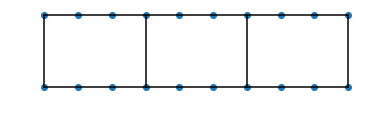
\includegraphics[scale=0.5]{picrel/first_block.png}
  \caption{Первый блок}
  \label{fig:first block}
\end{figure}

Если присоединить к нему кусочек, как на рисунке \ref{fig:2 blocks}, то плотность и максимальная плотность графа не изменятся.

\begin{figure}
  \centering
  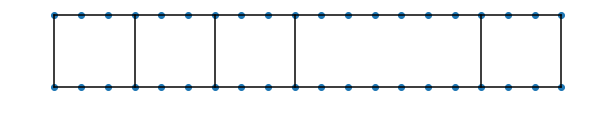
\includegraphics[scale=0.5]{picrel/2_blocks.png}
  \caption{Два блока}
  \label{fig:2 blocks}
\end{figure}

Можно присоединить 9 кусочков, увеличив число рёбер и 
вершин в десять раз, затем добавить (или не добавлять) одно ребро. Получившийся граф будет иметь вид, как граф на рисунке \ref{fig:additional edge}.

Таким способом можно увеличивать число рёбер и вершин в $10^k$ раз и добавлять ребро.
Последовательность плотностей графов будет стремиться к бесконечной апериодической десятичной дроби.

\begin{figure}
  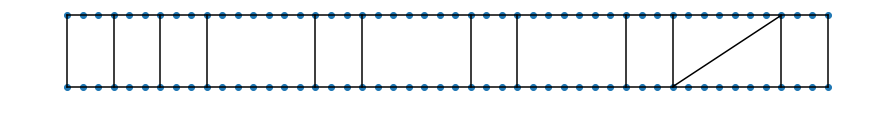
\includegraphics[scale=0.5]{picrel/additional_edge.png}
  \caption{Несколько блоков и дополнительное ребро}
  \label{fig:additional edge}
\end{figure}

Граф состоит из примыкающих друг к другу секций (кусочков), поэтому для записи формулы, выражающей существование этого или более плотного графа, достаточно столько переменных, сколько нужно, чтобы выразить существование наибольшей из секций.


Пусть $1/\alpha$~--- иррациональное число вида $1.1\{z_n\}_{n=1}^\infty$, где $\{z_n\}_{n=1}^\infty$~--- произвольная апериодическая последовательность нулей и единиц. Например, $1/\alpha = 1.101001000100001\ldots$~.
Определим для каждого $l \in \N$ граф $H_l$ следующим образом.
Для $l = 1$ граф $H_1$ с плотностью $\rho(H_1) = \rho^{max}(H_1) = 22/20 = 1.1$  уже определён.
Пусть $l > 1$.
С помощью приёма, описанного выше, увеличим число рёбер и вершин графа $H_1$ в 
%$l$ раз и дополнительно добавим $2\cdot(1/\alpha - 1.1)\cdot 10^{[\log_{10}l]}$ рёбер
$10^{l-1}$ раз и дополнительно добавим $[2\cdot(1/\alpha - 1.1)\cdot 10^{l}]$ рёбер.
Здесь необходимо выбрать такое правило добавления дополнительных рёбер, чтобы была справедлива лемма \ref{lem:balanced}.
Пока оставим эту техническую проблему в стороне и двинемся дальше, считая, что условие леммы \ref{lem:balanced} выполнено.

\begin{Lem}
\label{lem:balanced}
$\forall l \in \N $ граф $H_l$ строго сбалансирован.
\end{Lem}

Аналогично тому, как в разделе \ref{sec:triangles} для графа $H_{ksm}$ была определена формула $\varphi_{ksm}$, определим для графа $H_l$ формулу $\varphi_l$.
Мы не описываем здесь точный вид этой формулы, поскольку нам от неё важно лишь то, чтобы она была а.п.н. верна, если случайный граф содержит $H_l$, удовлетворяла лемме \ref{lem:density_irrational} и записывалась с помощью равномерно ограниченного по $l$ числа переменных. 
При этом представить себе формулу, удовлетворяющую первому и последнему требованиям, несложно, а лемма \ref{lem:density_irrational} нами не доказана, но мы считаем, что её утверждение довольно естественно.

\begin{Lem} 
\label{lem:density_irrational}
Если для графа $G$ истинна $\varphi_l$, и $G$ не содержит подграфа, изоморфоного $H_l$, то $G$ содержит более плотный подграф с меньшим числом вершин.
\end{Lem}

% И тут мы сталкиваемся с проблемой~--- леммы \ref{lem:density_irrational} не достаточно для того, чтобы было истинно $\neg \left( \Gna \vDash \varphi_{N'}\right),~ N' > N$.
% Поскольку ни теорема \ref{th:ruchinski}, ни другие известные нам результаты не дают гарантий того, что $\Gna$ не содержит (с близкой к 1 вероятностью) большого (например, содержащего $N/2$ вершин) подграфа $\tilde H$ с $\rho(\tilde H) > 1/\alpha$, то мы не можем быть уверены в том, что для $\Gna$ ложна $\varphi_{N'},~ N' > N$, т.к. $\varphi_{N'}$ может быть истинна для некоторого плотного графа $\tilde H$ с количеством вершин, меньшим $N$.

% Можно попробовать решить эту проблему, добавив для каждой переменной формулы $\varphi_l$ условие, что она не соответствует никакой другой позиции графа $H_l$.
% Действительно, если $G \vDash \varphi_{N'},~ N' > N$, то в $G$ есть вершина, которой соответствуют более одной переменной* формулы  $\varphi_{N'}$. Тем не менее, вводя такие ограничения, нужно убедиться, что они не сильно уменьшают вероятность истинности формулы, в том случае, когда $H_l$ действительно содержится в $\Gna$.

% Если если эта проблема решена, то 
Следующий шаг состоит в построении множества интервалов $\{[a_{2i}, a_{2i+1}] ~ | ~ i \in \N \}$.
Будем строить его таким образом, чтобы $a_1 < a_2 < a_3 < \ldots$.

Из теоремы \ref{th:ruchinski} следует, что для любого $v$ существует число $N_{v}$ такое, что $G\left(N_{v}, N_{v}^{-\alpha}\right)$ содержит копию любого графа с $\rho^{max} < 1/\alpha$ на не более чем $v$ вершинах с вероятностью $> 0.99$.
По лемме \ref{lem:balanced} максимальная плотность всех графов из $\{H_l\}_{l=1}^\infty$ меньше $1/\alpha$.
Тогда с вероятностью $> 0.99$ при $N \in [N_{v_1}, 10N_{v_1}]$
наибольший граф из $\{H_l\}_{l=1}^\infty$, имеющий копию в $\Gna$, имеет вершин $v^{max} \in [v_1, 10N_{v_1}]$.
Положим $a_1 = v_1, ~ a_2 = 10N_{v_1}$.
Далее, при $N \in [N_{100N_{v_1}}, 10N_{100N_{v_1}})$
с вероятностью $> 0.99$ выполнено $v^{max} \in [100N_{v_1},  10N_{100N_{v_1}})$~--- этот интервал не будем включать в $A$.
Зато включим в $A$ отрезок $[a_3, a_4] =  [10N_{100N_{v_1}}, 10N_{10N_{100N_{v_1}}}] $: в него, с вероятностью $> 0.99$ попадает $v^{max}$ при $N \in [N_{10N_{100N_{v_1}}}, 10N_{10N_{100N_{v_1}}}]$.
И так продолжаем до бесконечности.

\begin{figure}
\tikz[scale=0.9, every node/.style={scale=0.9}] {
    \draw (-1.5, 0) node {$v^{max}$};
    \draw (-0.5,0) --  (14,0);
        \draw (0,0) node {\textbf[ };
            \draw (0, 0.5) node {$v_1$};
        \draw (3,0) node {\textbf] };
            \draw (3.3, 0.5) node {$10\bfN_{v_1}$};
        \draw (5,0) node {\textbf[ };
            \draw (5, 0.5) node {$100\bfN_{v_1}$};
        \draw (7.95,0) node {\textbf) };
        \draw (8,0) node {\textbf[ };
            \draw (8.7, 0.5) node {$10\bfN_{100\bfN_{v_1}}$};
        \draw (12.5,0) node {\textbf] };
            \draw (13.5, 0.5) node{$10\bfN_{10\bfN_{100\bfN_{v_1}}}$};
    \draw (-1.5, -2) node {$N$};
    \draw (-0.5,-2) --  (14,-2);
        \draw (2,-2) node {\textbf[ };
            \draw (2, -2.5) node {$\bfN_{v_1}$};
        \draw (3,-2) node {\textbf] };
            \draw (3.3, -2.5) node {$10 \bfN_{v_1}$};
        \draw (7,-2) node {\textbf[ };
            \draw (6.7, -2.5) node {$\bfN_{100\bfN_{v_1}}$};
        \draw (8,-2) node {\textbf) };
            \draw (8.7, -2.5) node {$10\bfN_{{100\bfN_{v_1}}}$};
        \draw (11,-2) node {\textbf[ };
            \draw (11, -2.5) node {$\bfN_{10\bfN_{100\bfN_{v_1}}}$};
        \draw (12.5,-2) node {\textbf] };
            \draw (13.5, -2.5) node {$10\bfN_{10\bfN_{100\bfN_{v_1}}}$};
            
    \draw[->, thick] (2.5, -1.8) -- node[midway, left] {$P>0.98$} (1.5, -0.2);
    \draw[->, thick] (7.5, -1.8) -- node[midway, left] {$P>0.98$} (6.5, -0.2);
    \draw[->, thick] (11.75, -1.8) -- node[midway, left] {$P>0.98$} (10.5, -0.2);
    \draw[decorate, decoration=snake, blue, thick] (0, 0) -- (3,0);
    \draw[decorate, decoration=snake, gray, thick] (5, 0) -- (8,0);
    \draw[decorate, decoration=snake, blue, thick] (8, 0) -- (12.5,0);
}
\caption{На верхней оси изображены интервалы $[a_i, a_{i+1}] \subset A$ (выделены голубым) и интервалы, исключенные из $A$ (выделены серым). На нижней оси изображены интервалы числа вершин случайного графа $\Gna$, на которых $v^{max}$ с высокой вероятностью принадлежит соответствующим интервалам на верхней оси }
\end{figure}


Пусть теперь $N'_v$~--- такое число, что при $N = N'_v$ случайный граф $\Gna$ с вероятностью $>0.99$ не содержит графов на не более чем $v$ вершинах с $\rho^{max} > 1/\alpha$.
Если положить $\mathbf{N}_v = \max\{N_v, N'_v\}$, и заменить в рассуждении выше $N_v$ на $\mathbf{N}_v$, то с помощью полученных таким образом интервалов можно построить формулу, вероятность истинности которой не будет иметь предела в $[0,1]$.
Действительно, при $N > \mathbf{N}_V$ по лемме \ref{lem:density_irrational} с вероятностью, превышающей $0.99$, свойство содержать $H_l$ равносильно истинности $\varphi_l$.
В последовательности $\{H\}_{l=1}^\infty$ между индексами $l$ и числом вершин $v_l$ существует однозначное соответствие и, по построению, $v_{l+1} = 10 v_l$.
Интервалы, входящие в $A$, а также интервалы, которые мы намеренно исключили из $A$, строились таким образом, чтобы их нижние границы отличались от верхних в $10$ раз, поэтому для каждого из этих интервалов существует индекс $l$ такой, что $v_l$ попадает в интервал.
Поэтому объединению интервалов числа вершин $A$ соответствует множество индексов $L$ такое, что вероятность истинности формулы \[
\bigvee_{l \in L} \varphi_l \wedge \neg \varphi_{l+1} 
\]
не имеет предела в $[0,1]$.

В этом рассуждении остаются пробелы в виде доказательств лемм \ref{lem:balanced}, \ref{lem:density_irrational}.
Если бы они были устранены, мы бы доказали, что в любой левой полуокрестности единицы существует иррациональное $\alpha$, для которого нарушается закон нуля или единицы для языка $\LL^k_{\infty, \omega}$ при некотором $k$ порядка $10$.
Далее можно было бы оптимизировать конструкцию, уменьшив число переменных в формуле $\varphi_l$ и доказать это утверждение для $k$ близкого или равного трём.